% -*- TeX:de -*-
\NeedsTeXFormat{LaTeX2e}
\documentclass[12pt,a4paper,titlepage]{article}

%\usepackage[german]{babel} % german text
\usepackage[DIV12]{typearea} % size of printable area
\usepackage[T1]{fontenc} % font encoding
\usepackage[utf8]{inputenc} % probably on Linux

\usepackage{graphicx} % to include images
\graphicspath{ {img/} } % set default image directory
\usepackage{subfigure} % for creating subfigures
\usepackage{amsmath} % a bunch of symbols
\usepackage{amssymb} % even more symbols
\usepackage{booktabs} % pretty tables
\usepackage{csquotes}

% a floating environment for circuits
\usepackage{float}
\usepackage{caption}

\newfloat{circuit}{tbph}{circuits}
\floatname{circuit}{Schaltplan}

% a floating environment for diagrams
\newfloat{diagram}{tbph}{diagrams}
\floatname{diagram}{Diagramm}

\renewcommand{\familydefault}{\sfdefault} % activate to use sans-serif font as default

\sloppy % friendly typesetting

\usepackage{eurosym}
\usepackage{makeidx}
\usepackage{amsfonts}
\usepackage{mparhack}
\usepackage{array}
\usepackage{tabularx}
\usepackage{minitoc}
\usepackage[colorlinks=true]{hyperref}
\usepackage{epstopdf}
\usepackage{setspace}
\usepackage{csquotes}

% hyperref settings
\hypersetup{
    colorlinks=false,       % false: boxed links; true: colored links
    linkcolor=black,          % color of internal links (change box color with linkbordercolor)
    citecolor=black,        % color of links to bibliography
    filecolor=black,      % color of file links
    urlcolor=black           % color of external links
}

\begin{document}

\begin{titlepage}

\begin{figure*}[h!]
  
\includegraphics[width=8cm]{TULogo_CMYK}
\end{figure*}

\begin{center}
\vspace*{1.3cm}
{\Huge Elektrotechnische Grundlagen der Informatik\\(LU 182.692)\\}
\vspace{1.7cm}
{\LARGE Protokoll der 3. Laborübung: \enquote{Operationsverstärker}\\}
{\LARGE  a) LTSPICE-Simulationen\\}
\vspace{1.7cm}

% fill in group number and date of lab here
% CHANGE ME!
{\Large Gruppennr.: 22 \hspace{1cm} Datum der Labor\"ubung: 01.06.2017}

% fill in IDs and names here
% CHANGE ME!
\begin{table}[h!]
\centering
\begin{tabular}{|p{3.5cm}|p{3.5cm}|p{6.5cm}|}
\hline \textbf{Matr. Nr.} & \textbf{Kennzahl} & \textbf{Name} \\
\hline
1614835 & 033 535 & Jan Nausner \\
\hline
1633068 & 033 535 & David Pernerstorfer \\
\hline
\end{tabular}
\end{table}

\end{center}
\vspace{1.0cm}

\begin{table}[h!]
\begin{tabular}{|l|l|}
\hline \textbf{Kontrolle} & \checkmark \\
\hline Nichtinvertierender OPV & \\
\hline OPV und Grenzfrequenz & \\
\hline Invertierender OPV & \\
\hline Integrierer & \\
\hline Schmitt-Trigger & \\
\hline
\end{tabular}
\end{table}

\end{titlepage}
% start of actual lab protocol
% CHANGE ME!

\setcounter{page}{2}

\newpage
\setcounter{tocdepth}{1}
\tableofcontents

\newpage



\section{Nichtinvertierender Verst\"rker}

\subsection{Aufgabenstellung}
Das Verhalten eines OPV als nichtinvertierender Verst\"arker soll mittels LTSpice simuliert werden.

\subsection{Schaltplan}
\begin{figure}[H]
  \centering
  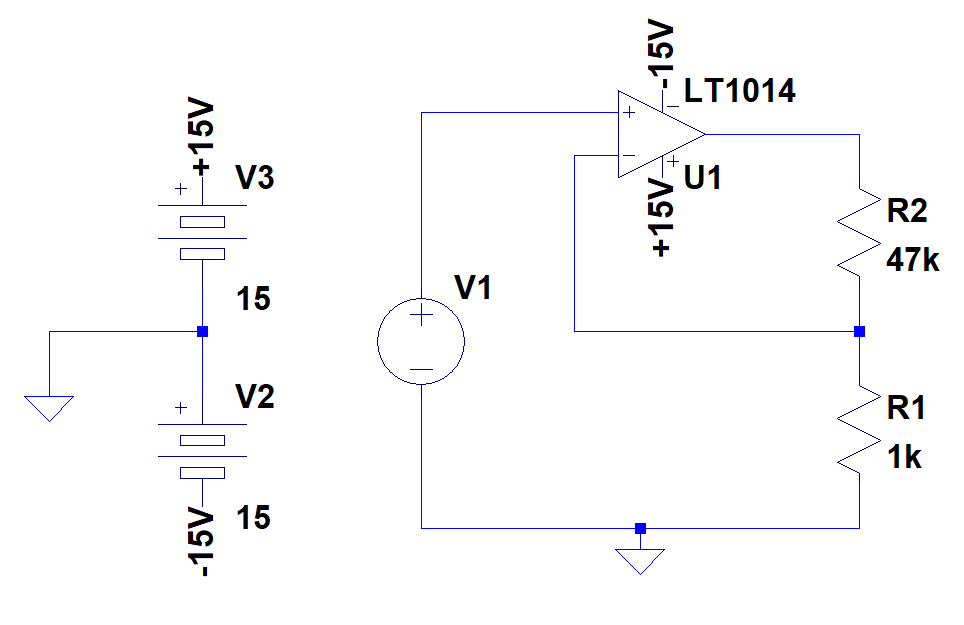
\includegraphics{nichtinvertierend_schaltung}
  \caption{Nichtinvertierender Verst\"arker}
%  \label{figure01}
\end{figure}

\subsection{Durchf\"uhrung}
Die Schaltung eines OPV als nichtinvertierender Verst\"arker wurde mit LTSpice aufgebaut. Die Spannungsverst\"arkung wird mit $V_u = 1 + \frac{R_2}{R_1}$ berechnet und soll zwischen 40 und 60 liegen. Das bedeutet $R_2$ muss etwa 40 bis 60 mal gr\"o\ss er dimensioniert werden als $R_1$. Gew\"ahlt wurden die Widerst\"ande $R_1 = 1k\Omega$ und $R_2 = 47k\Omega$. Nun wurde das Verhalten des Systems mit einer DC Eingangsspannung bzw. mit 2 verschieden Rechteckspannungen (siehe Angabe) simuliert und diverse Messungen durchgef\"uhrt (siehe Ergebnis \& Diskussion).


\subsection{Ergebnis \& Diskussion}
\begin{figure}
  \centering
  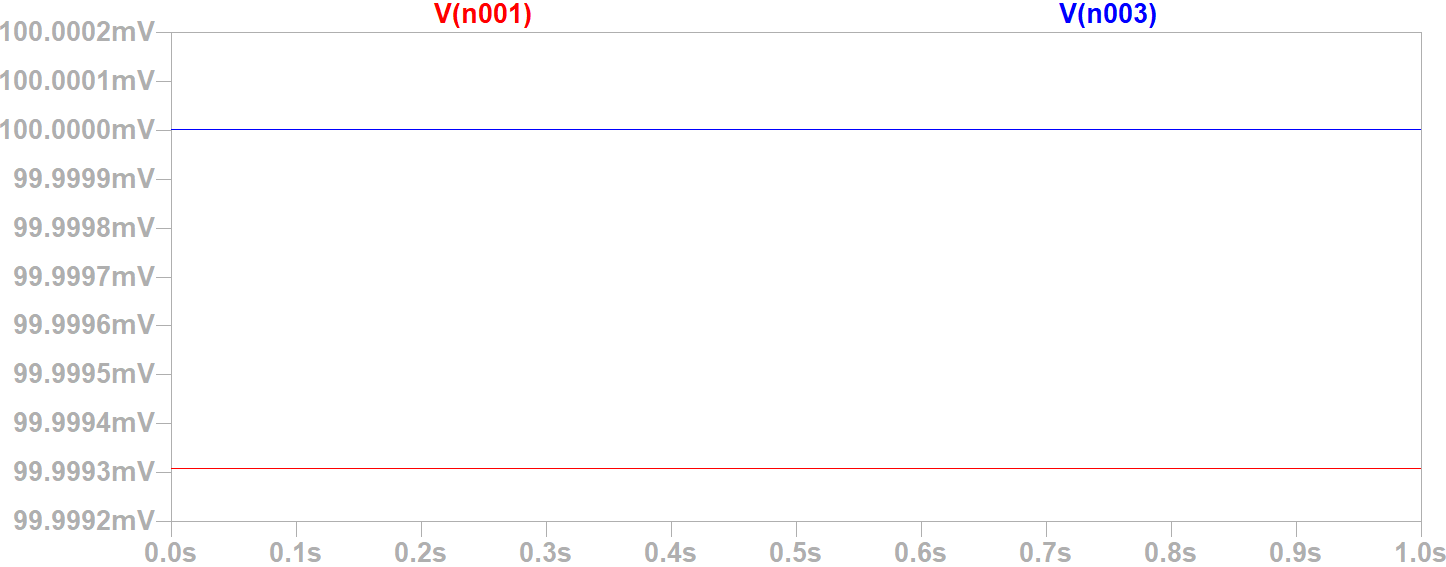
\includegraphics[width=150mm]{nichtinvertierend_dc_eingaenge_spannungen}
  \caption{Nichtinvertierender Verst\"arker; Blau: $U_p$; Rot: $U_n$}
  \label{figure01}
\end{figure}
In Abbildung~\ref{figure01} sind die Spannungen des positiven ($U_p$) und negativen ($U_n$) Einganges des OPV zu sehen. $U_p$ entspricht klarerweise der Eingangsspannung $U_e$. Da zwischen den beiden Eing\"angen  


\section{Invertierender Verst\"rker}

\subsection{Aufgabenstellung}

\subsection{Schaltplan}

\subsection{Durchf\"uhrung}

\subsection{Ergebnis \& Diskussion}

\section{Integrierer}

\subsection{Aufgabenstellung}
Das Verhalten eines Integrierers soll im Zeit- und Frequenzbereich simuliert werden.

\subsection{Schaltplan}
\begin{figure}[H]
  \centering
  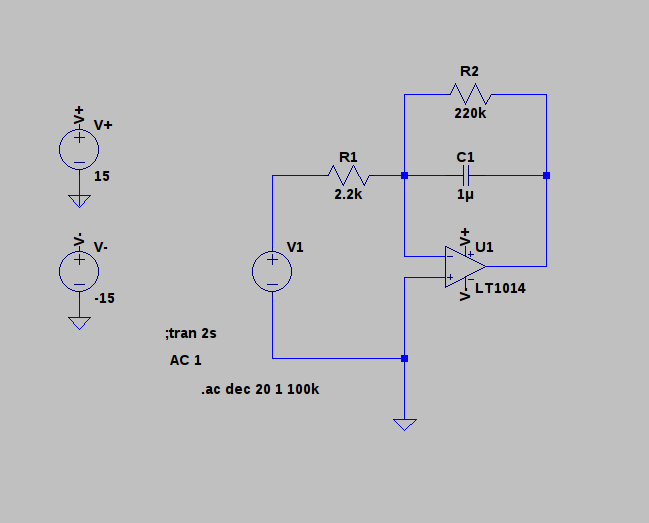
\includegraphics[width=100mm]{integrierer_schaltung.png}
  \caption{Integrierer}
\end{figure}

\subsection{Durchf\"uhrung}
Die Schaltung wurde gem\"aß Angabe zusammengef\"ugt. Die Versorgungsspannung des OPV (LT1014) betr\"agt $\pm 15V$. Um das Verhalten im Zeitbereich zu simulieren, wurde eine Rechteckspannung mit $f=5Hz, A=\pm 0,1V, V_{initial}=-0,1V$ angelegt. Das Zeitverhalten wurde im Bereich von $0$ bis $2s$ aufgezeichnet. Zur Simulation des Frequenzverhaltens wurde eine Sinusspannung mit $1V_{pp}$ angelegt und das Bode-Diagramm von $1Hz-100kHz$ aufgezeichnet.

\subsection{Ergebnis \& Diskussion}

\begin{figure}[H]
  \centering
  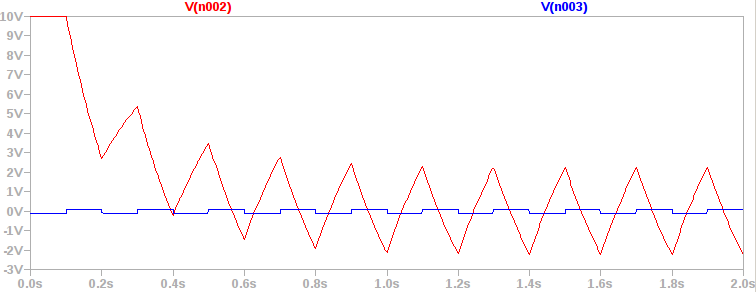
\includegraphics[width=150mm]{integrierer_transient.png}
  \caption{Zeitverhalten (rot $\hdots$ Ausgangsspannung, blau $\hdots$ Eingangsspannung)}
\end{figure}
Im Bereich von $0$ bis $1s$ ist ein Einschwingvorgang zu erkennen, welcher auf das $RC$-Glied zur\"uckzuf\"uhren ist. Da die Differenz der beiden OPV-Eing\"ange zu Beginn $-0,1V$ Betr\"agt, \"ubersteuert der OPV, die Differenz schl\"agt auf $0,1V$ um und der OPV versucht zu untersteuern, dann pendelt sich das Signal ein. Im eingeschwungenenen Zustand wird das anliegende Rechtecksignal gem\"aß der \"Ubertragungsfunktion

\begin{figure}[H]
  \centering
  $U_a = -\frac{1}{RC}\int U_e dt$
\end{figure}

\noindent zu einem Dreieckssignal mit

\begin{figure}[H]
  \centering
  $U_e<0: U_a = \frac{t}{10*RC} \approx 45,5*t, U_e>0: U_a = -\frac{t}{10*RC} \approx -45,5*t$
\end{figure}

\noindent integriert. TODO: Anfangsbedingung, Vpp!!!


\begin{figure}[H]
  \centering
  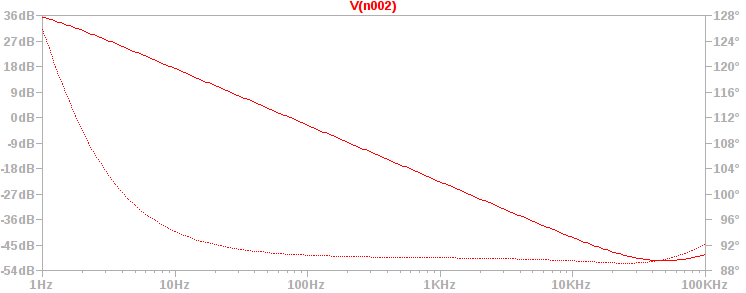
\includegraphics[width=150mm]{integrierer_bode.png}
  \caption{Bode-Diagramm}
\end{figure}

\noindent Am Frequenzverhalten kann man erkennen, dass das System bis zur Grenzfrequenz des $RC$-Glieds ($f_g = \frac{1}{2\pi RC} \approx 72Hz$) verst\"arkend wirkt und danach zu D\"ampfen beginnt. Die Filtersteilheit betr\"agt $-20dB/Dekade$. Die Phase dreht zuerst sehr stark, dann immer schw\"acher von $126^{\circ}$ auf $90^{\circ}$. Im Bereich \"uber $40kHz$ beginnt die Phasenverschiebung wieder zu steigen und die D\"ampfung wird schw\"acher.

\section{Invertierender Schmitt-Trigger}

\subsection{Aufgabenstellung}
Das Verhalten eines invertierenden Schmitt-Triggers soll im Zeitbereich simuliert werden.

\subsection{Schaltplan}
\begin{figure}[H]
  \centering
  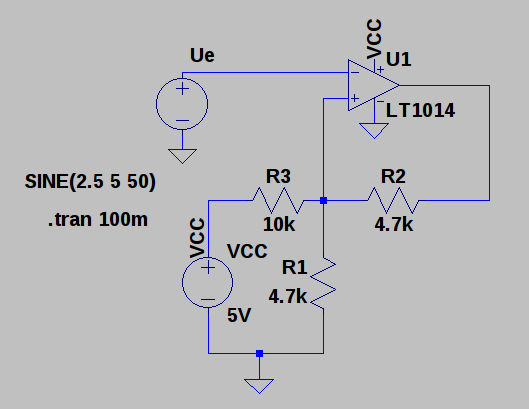
\includegraphics[width=100mm]{schmitt_schaltung.png}
  \caption{Invertierender Schmitt-Trigger}
\end{figure}

\subsection{Durchf\"uhrung}
Die Schaltung wurde gem\"aß Angabe zusammengef\"ugt. Die Versorgungsspannung des OPV (LT1014) betr\"agt $V+=5V,V-=0V$. Zuerst wurde die Aus- und Eingangsspannung, sowie die Spannung am positiven Eingang des OPV im Bereich von $0$ bis $100ms$ mit einem Sinus-Eingangssignal ($DC_{offset} = 2,5V, V_{pp} = 5V, f = 50Hz$) simuliert. Dann wurde das Zeitverhalten mit einem Dreieckssignal ($V_{on} = 5V, V_{off} = 0V, f = 5MHz$) von $0$ bis $1\mu s$ simuliert.

\subsection{Ergebnis \& Diskussion}

\begin{figure}[H]
  \centering
  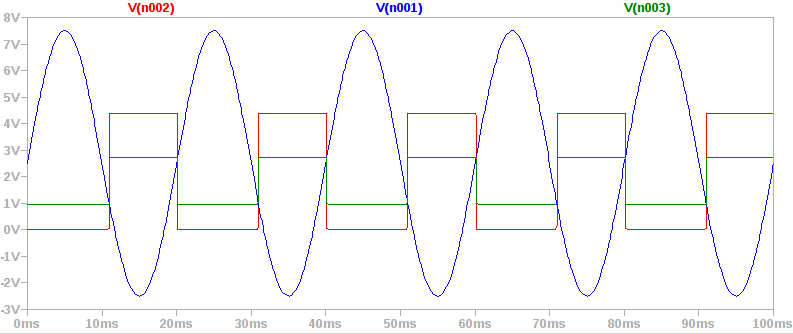
\includegraphics[width=150mm]{schmitt_transient.png}
  \caption{Zeitverhalten bei Sinussignal (rot $\hdots$ Ausgangsspannung, blau $\hdots$ Eingangsspannung, gr\"un $\hdots$ Spannung am positiven OPV Eingang)}
\end{figure}

\noindent Berechnung der Spannung am positiven OPV Eingang mittels Superpositionsprinzip:

\begin{itemize}
  \item $U_{low} = 0,029V$ (abgelesen):\\
  $U_a$ kurzgeschlossen:\\
  $U_{p1} = U_{VCC}\frac{R_{12}}{R_{12}+r_3} = U_{VCC}\frac{\frac{R_1R_2}{R_1+R_2}}{\frac{R_1R_2}{R_1+R_2}+R_3} = 5V\frac{2,35k\Omega}{2,35k\Omega + 10k\Omega} \approx 0,95V$\\
  $U_{VCC}$ kurzgeschlossen:\\
  $U_{p2} = U_{low}\frac{R_{13}}{R_{13}+R_2} = U_{low}\frac{\frac{R_1R_3}{R_1+R_3}}{\frac{R_1R_3}{R_1+R_3}+R_2} = 0,029V\frac{3,19k\Omega}{3,19k\Omega + 4,7k\Omega} \approx 0,01V$\\
  $U_p = U_{p1} + U_{p2} \approx 0,96V$

  \item $U_{high} = 4,39V$ (abgelesen):\\
  $U_a$ kurzgeschlossen:\\
  $U_{p1} = U_{VCC}\frac{R_{12}}{R_{12}+R_3} = U_{VCC}\frac{\frac{R_1R_2}{R_1+R_2}}{\frac{R_1R_2}{R_1+R_2}+R_3} = 5V\frac{2,35k\Omega}{2,35k\Omega + 10k\Omega} \approx 0,95V$\\
  $U_{VCC}$ kurzgeschlossen:\\
  $U_{p2} = U_{high}\frac{R_{13}}{R_{13}+R_2} = U_{high}\frac{\frac{R_1R_3}{R_1+R_3}}{\frac{R_1R_3}{R_1+R_3}+R_2} = 4,39V\frac{3,19k\Omega}{3,19k\Omega + 4,7k\Omega} \approx 1,78V$\\
  $U_p = U_{p1} + U_{p2} \approx 2,73V$
\end{itemize}

\noindent Die Spannung am positiven Eingang des OPV bestimmt (wie auch im Diagramm ersichtlich), wann getriggert wird. Das heißt, wenn das Sinussignal am Eingang unter $0,95V$ f\"allt, liefert der OPV am Ausgang $U_{high}$, wenn das Eingangssignal $2,73V$ \"ubersteigt, liegt am Ausgang $U_{low}$ an. Somit wandelt der Schmitt-Trigger das Sinussignal in ein invertiertes Rechtecksignal um.

\begin{figure}[H]
  \centering
  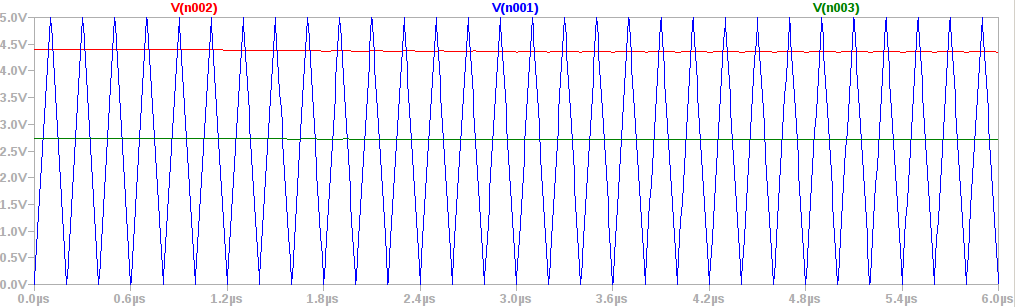
\includegraphics[width=150mm]{schmitt_transient_final.png}
  \caption{Zeitverhalten bei $5MHz$ Dreieckssignal (rot $\hdots$ Ausgangsspannung, blau $\hdots$ Eingangsspannung, gr\"un $\hdots$ Spannung am positiven OPV Eingang)}
\end{figure}

\noindent TODO: Interpretation

\end{document}
